\section{Introduction}
\label{sec:intro}

Active automata learning aims to construct black-box state diagram models of software and hardware systems
by providing inputs and observing outputs.
In 1987, Angluin \cite{Ang87} published a seminal paper in which she showed that finite automata can be learned using so-called 
\emph{membership queries} and \emph{equivalence queries}.
Many (if not most) efficient active learning algorithms used
today are designed following Angluin's approach of a \emph{minimally adequate teacher (MAT)}.
In this approach, learning is viewed as a game in which a learner has to infer the behavior of
an unknown state diagram by asking queries to a teacher.
Following pioneering work by \cite{Ang87,PeVaYa02,Hagerer2002,RaMeSM2009,IsHoSt2015},
active automata learning is emerging as an effective bug finding technique.
Using active automata learning, for instance, standard violations have been found in many implementations of
major network and security protocols such as TLS \cite{dRP15}, TCP \cite{FJV16,FH17} and SSH \cite{FiterauEtAl17}.

Timing often plays a crucial role in these applications.
A TCP implementation, for instance, may retransmit packets if they are not acknowledged within
a specified time. Also, a timeout may occur if the implementation does not receive an acknowledgment
after a number of retransmissions, or if it remains in certain states too long.
Timing behavior cannot be captured using existing learning tools, which only support learning of deterministic
Mealy machines and related untimed models.
In the case of TCP, previous work only succeeded to learn Mealy machine models by having the network adaptor 
ignore all retransmissions, and by completing learning queries before the occurrence of certain timeouts \cite{FJV16}.
All timing issues had to be artificially suppressed.

There has been some work on algorithms for learning timed systems, e.g., \cite{GrinchteinJP06,GrinchteinJL10,CCF16,VWW:rti}.
The modeling frameworks of \cite{VWW:rti,CCF16} are very restrictive however: they essentially allow only a single timer, which is reset on every transition,
thus allowing to represent only constraints on delays between successive transitions. In contrast, the event recording automata studied by \cite{GrinchteinJP06,GrinchteinJL10} appear to have too many degrees of freedom, leading to
prohibitively complex the learning algorithms.
%% For learning, we would like to have a class of models where the occurrence of timing-dependent behavior
%% is determined by previous behavior, that is, fewer degrees of freedom than what is supported by event-recording automata.
In the literature, there is no tractable algorithm which can learn models of
common network protocols which also captures their timing aspects, including
setting and expiration of timers.

In this paper, we address this challenge by presenting a framework for learning
timed extensions of automata models that appear to
be sufficiently expressive to describe the real-time behavior of network protocols such as TLS, TCP and SSH.
%
Our work is inspired by the results of \cite{CCF16} on time delay Mealy machines,
but we focus on a significantly richer class of automata models.
We introduce the class of Mealy machines with timers (MMTs) that is able to
model the timing behavior of a wide variety of communication protocols.
Timers are set to integer values in transitions, and may be stopped or
time out in later transitions.
%%  We assume that
%% each timeout immediately triggers an observable output, implying that
%% we can observe the occurrence of a timeout indirectly. However, we cannot observe which timer times out.
MMTs can be viewed as a formalization of the finite state models with countdown timers that are used in the textbook of
Kurose and Ross \cite{KR13} to explain transport layer protocols.
Figure~\ref{fig:abp} presents an MMT model of the sender from 
the alternating-bit protocol, adapted from \cite[Figure 3.15]{KR13}.
\begin{figure}[h]
\centering
\begin{tikzpicture}[->,>=stealth',shorten >=1pt,auto,node distance=2.3cm,main node/.style={circle,draw,font=\sffamily\large\bfseries}]
  \node[initial, state] (1) {$q_0$};
  \node[state] (2) [right of=1] {$q_1$};
  \node[state] (3) [below of=2] {$q_2$};
  \node[state] (4) [below of=1] {$q_3$};

  \path[every node/.style={font=\sffamily\scriptsize}]
    (1) edge [text width=1.5cm] node {$\mathit{in}/\mathit{send0}$ \\ $x := 3$} (2)
    (2) edge [text width=1.5cm] node {$\mathit{ack0}/\Lambda$ \\ $\mathit{stop}(x)$} (3)
        edge [loop right, text width=1.5cm] node {$\toevent{x}/\mathit{send0}$\\ $x := 3$ } (2)
    (3) edge [text width=1.5cm] node {$\mathit{in}/\mathit{send1}$ \\ $x := 3$} (4)
    (4) edge [text width=1cm] node {$\mathit{ack1}/\Lambda$ \\ $\mathit{stop}(x)$} (1)
        edge [loop left, text width=1.5cm] node {$\toevent{x}/\mathit{send1}$\\ $x := 3$} (4);
\end{tikzpicture}
\caption{MMT model for alternating-bit protocol sender}
\label{fig:abp}
\end{figure}
In the diagram $x :=3$ denotes that a transition starts a timer $x$ with value $3$,
and $\mathit{stop}(x)$ denotes that timer $x$ is stopped.
For readability we have omitted trivial self-loops.
The approaches of \cite{VWW:rti,CCF16} cannot model this protocol.
\iflong
$\Lambda$ denotes the absence of an observable output. 

%\todobj{I think we do not have space for this explanation}
%In the model, input $\mathit{in}$ corresponds to a request from the upper layer to transmit data.
%Initially, upon receipt of such a request, the sender builds a packet from the data and a sequence number $0$,
%sends the packet over the network (output $\mathit{send0}$), and starts the timer with timeout value $3$.
%If the sender receives an acknowledgment with the right sequence number $0$ (input $\mathit{ack0}$) 
%then it stops the timer and jumps to state $q_2$.
%Acknowledgment with the incorrect sequence number (input $\mathit{ack1}$) are ignored.
%If no $\mathit{ack0}$ input arrives within $3$ time units, a timeout occurs and the same packet is sent again.
%The behavior in states $q_2$ and state $q_3$ is analogous to that in states $q_0$ and $q_1$, respectively,
%with the roles of $0$ and $1$ swapped.
\fi

We present a natural timed adaptation of the MAT framework for learning MMTs.
We base it on the set of {\em timed words} of an MMT, which record possible
sequences of inputs and outputs and their precise timing.
In an MMT, each timeout immediately triggers an observable output, hence
we can observe the occurrence of a timeout indirectly. However,
we cannot observe which timer times out.
In a membership query, the learner supplies a sequence of inputs with
precise timing.
In response, the teacher specifies outputs occur in response to these inputs,
as well as their precise timing.
Via an equivalence query, the learner asks whether a hypothesis MMT that it has
constructed accepts the same timed words
as the (unknown) MMT of the teacher. If this is the case,
the teacher's answer is `yes';
otherwise it is `no' coupled with a timed word showing that the
hypothesis is incorrect.

The timed MAT framework naturally corresponds to a setting, where the behavior
of a black-box protocol component is investigated by supplying inputs. However,
it is not convenient for formulating model learning algorithms. We therefore
develop an alternative semantics for MMTs, based on sets of {\em untimed words},
which do not record timing of inputs and outputs, but instead record when and how timers are set and when they expire. We show, perhaps surprisingly, that
under certain mild restrictions (the most important being that each transition
sets at most one timer) this untimed semantics is equivalent to the above
timed semantics. The result shows that the set of timed words can be inferred
from the set of untimed words and vice versa.
%\todobj{Should the following sentence really be included?}
%Intuitively, causality of timeouts can be inferred in the timed semantics since a slight change in the timing of an input event leads to a corresponding change in the timing of any timeout that it induces.

The result of Section 3 suggests an architecture for our active learning algorithm that is shown in Figure~\ref{architecture}.
The idea is to define an alternative (and simpler) MAT framework in which the learner uses membership queries (MQ) and equivalence queries (EQ)
to obtain information about the untimed behaviors of an MMT.
An adapter then implements each untimed membership query via a series of timed membership queries for the timed teacher,
and each untimed equivalence query via a timed equivalence query.
From the perspective of an untimed learner, the combination of the adapter and a timed teacher acts like an untimed teacher.
Conversely, the combination of an untimed learner and the adapter behaves like a timed learner.
\begin{figure}[h]
\begin{center}
 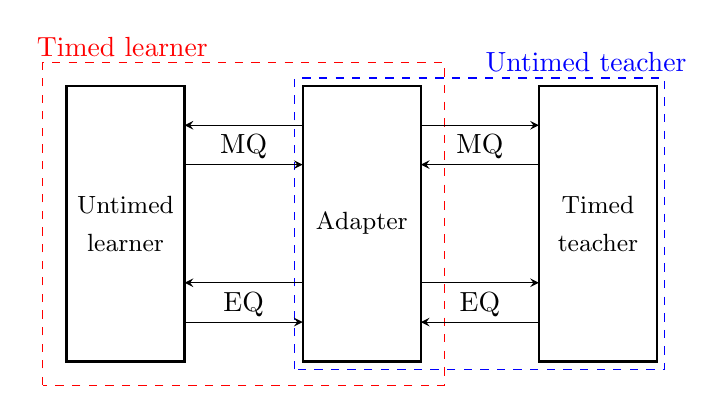
\begin{tikzpicture}[>=stealth]
 \draw [dashed,red] (-3.3,-0.3) rectangle (1.8,3.8);
 \node [above,right,red] at (-3.5,4) {Timed learner};
 \draw [dashed,blue] (-0.1,-0.1) rectangle (4.6,3.6);
 \node [above,right,blue] at (2.2,3.8) {Untimed teacher};
            \draw [thick] (0,0) rectangle (1.5,3.5) node[midway] {\small Adapter};
            \draw [thick] (3,0) rectangle (4.5,3.5) node[midway,above] {\small Timed};
            \draw [thick] (3,0) rectangle (4.5,3.5) node[midway,below] {\small teacher};
            \draw [->] (1.5,3) -- (3,3) node[midway,below] {MQ};
            \draw [<-] (1.5,2.5) -- (3,2.5);
            \draw [->] (1.5,1) -- (3,1) node[midway,below] {EQ};
            \draw [<-] (1.5,0.5) -- (3,0.5);
            \draw [->] (0,3) -- (-1.5,3) node[midway,below] {MQ};
            \draw [<-] (0,2.5) -- (-1.5,2.5);
            \draw [->] (0,1) -- (-1.5,1) node[midway,below] {EQ};
            \draw [<-] (0,0.5) -- (-1.5,0.5);
            \draw [thick] (-3,0) rectangle (-1.5,3.5) node[midway,above] {\small Untimed};
            \draw [thick] (-3,0) rectangle (-1.5,3.5) node[midway,below] {\small learner};
        \end{tikzpicture}
\end{center}
\caption{Learning architecture}
\label{architecture}
\end{figure}

In order to develop a learning algorithm for the untimed MAT framework, we first develop
a Nerode equivalence, which generalizes the standard Nerode equivalence for
regular languages, and induces the canonical MMTs that will be constructed by the learning algorithm. 
We also develop an approximation of this Nerode equivalence,
parameterized by sets of suffixes, which is the basis for constructing
hypothesis automata in the learning algorithm. The approximated Nerode
equivalence allows us finally to present an active automata learning
algorithm for MMTs. This algorithm allows to learn MMTs using a number
of membership and equivalence queries, which is polynomial in the number of
states of the resulting MMT, and doubly exponential in the maximal number of
simultaneously active timers.

To summarize, our paper includes the following contributions:
\begin{itemize}
\item
  a new model of timed systems, MMTs, which is a small extensions of Mealy machines, but still expressive enough for many network protocols,
  \item
    an untimed semantics equivalent to the timed semantics for MMTs, which allows
    to define a Nerode equivalence as a basis for learning algorithms
   \item
     a tractable automata learning algorithm for learning MMTs.
\todobj{Should this be made more precise?}
\end{itemize}

In Section~\ref{sec:mmt}, we present the definition of MMTs, their timed semantics, and a minimally adequate teacher for MMTs.
Section~\ref{section untimed semantics} presents the untimed semantics, and the
equivalence with the timed semantics.
Section~\ref{algorithm} describes the untimed MAT framework for MMTs and the adapter that implements an untimed teacher using a timed teacher.
Section~\ref{sec:nerode} presents the Nerode equivalence and its approximated
version, and
Section~\ref{sec:learning} presents our learning algorithm.
Section~\ref{conclusions} contains some concluding remarks and lists topics for future research.
\ifshort
A full version of this article including proofs is available at \url{http://www.sws.cs.ru.nl/publications/papers/fvaan/MMT}.
\fi

\paragraph{Related Work}
Previous work on learning timed automata models have either been very complex, and not suitable as a basis for
practical implementation~\cite{GrinchteinJP06,GrinchteinJL10}, one reason being that they aim to learn rather
general classes of models, or target rather restricted models, e.g., allowing to capture only
delays between consecutive transitions~\cite{VWW:rti,VWW:ic11}. 
There are also algorithms for learning timed models from white-box components,
whose internal ``code'' can be inspected~\cite{lin2014learning} and whose
internal state can be inspected during execution~\cite{maier2014online}.

Other generalizations of classical automata learning include algorithms for
learning of symbolic automata~\cite{MensM15,Drews:tacas17}
or register automata~\cite{BLP:remember,HoStMe2011,HowarSJC12,CasselHJS16}.
These models
can capture simple relations, such as equality and ordering,
between data parameters of inputs and outputs, but cannot capture how
timers operate. The techniques for learning them cannot be applied to
MMTs, although our treatment of unknown timer names has been inspired by
their handling of unknown registers names.
The treatment of timer names in our Nerode equivalence has also been inspired
by treatment of registers in corresponding equivalences for register automata
\cite{CasselHJMS15}.
